The implementation of the alternative heuristics is based on the improvements
made by~\cite{devriendt2012symmetry} based on the MiniSAT SAT-solver.
In order to ease the testing procedure and overall usage of the solver, all heuristics
are implemented within the same program. One may choose one or multiple heuristics
by using command line parameters. Because of this feature it is possible to combine
multiple heuristics into a new heuristic.
While benchmarking we disabled the built-in heuristic that randomly chooses a literal from the heap,
such that our results are fully deterministic.
Further combinations of heuristics are not tested because this falls outside the scope
of this research.

We will analyze the results for each of the heuristics separately and discuss for each of them both
hypothesis as formulated in section \ref{sec:Introduction}.
Beforehand we discuss some results that are observed for each of the measured heuristics.

\subsection{Generic Results}
	Firstly, it is observed that $SP^{REG}$ and $SP^{OPT}$ perform equally on all measured sets,
	except Urquhart.
	This conforms to our expectations, as the only difference between these implementations is the
	optimizing heuristic for inverting symmetries, and only the Urquhart set contains inverting
	symmetries in our selection of benchmarks.

	It is observed in the activity data that none of implementations, including $SP^{OPT}$,
	succeeds in increasing the number of active symmetries in the CHNL benchmark suite.

	The same is true for the Urquhart benchmarks.
	This however was to be expected, as it only contains inverting symmetries.
	The searcher therefor picks a branch literal (that is expected to keep more symmetries active),
	but during symmetry propagation, the weakly active symmetry would be made permanently inactive
	because it contains literals that invert under the symmetry.

	One might expect that SA would perform as good as $SP^{OPT}$ under these circumstances.
	However, our implementation only performs \emph{unit propagation} during the lookahead, such
	that inverting symmetries are counted as active during the lookahead.

\subsection{SA Heuristic}
	From a theoretical perspective, SA was expected to have the most impact on the number of active
	symmetries during search, as it optimizes is very directly using a one iteration lookahead.
	This is reflected in the measured active symmetries.
	From all four heuristics, the SA heuristic is the one that performs best on this metric.

	The most prominent result is that it performs better (on the activity metric) than $SP^{OPT}$ in
	all but two battleship instances.
	Additionally, it keeps more symmetries active in the all of the shuffled pigeonhole benchmarks
	than $SP^{OPT}$.
	The first hypothesis is therefor true for the SA heuristic.

	When we look at the performance, however, there seems to be no correlation
	between the number of active symmetries and the number of decisions.
	This is made more clear by the scatter plot in figure \ref{fig:correlation}.
	If an increased amount of weakly active symmetries would have resulted in better performance in
	general and vice versa, than the scatter plot should have shown some increasing line (it can be
	seen that this is the case for $SP^{OPT}$).

	It is crucial to recall that SA chooses from the top five variables on the variable heap and
	does not alter anything else in the solver.
	The weakest conclusion that one can draw from this is that SA is not a better heuristic than the
	built-in VSIDS heuristic.
	The strongest conclusion would be to reject hypothesis 2, which we will discuss in
	\ref{ssec:falsification_hyp_2}.

	\begin{figure*}[!ht]
		\center
		\centerline{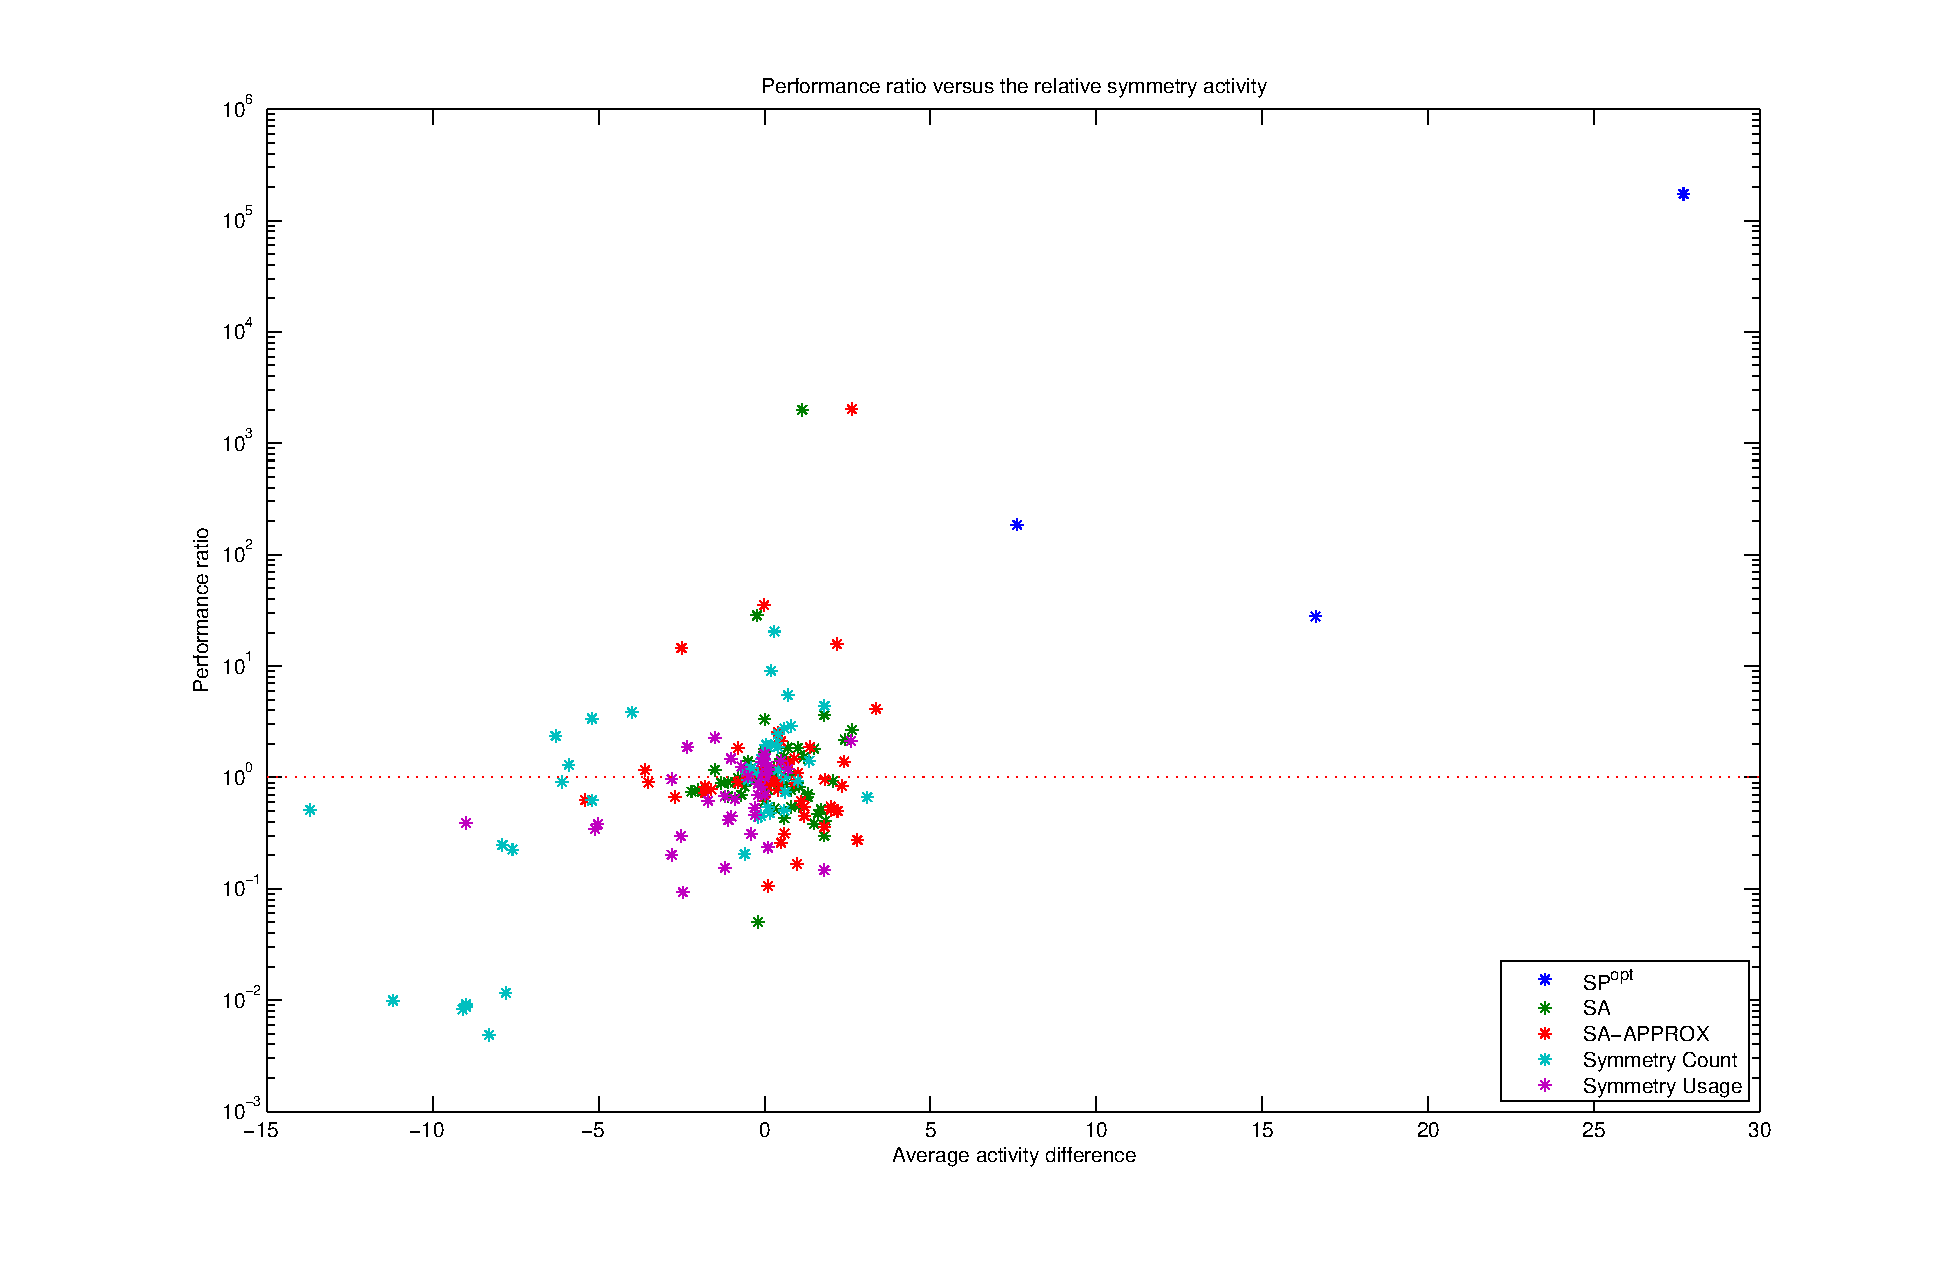
\includegraphics[width=1.2\textwidth]{results/scatterplot_activity.eps}}
		\caption{
			Correlation between number of active symmetries and number of decisions for all
			heuristics. Performance and activity measured relative to $SP^{REG}$.
		}
		\label{fig:correlation}
	\end{figure*}

\subsection{SC Heuristic}
	The symmetry count heuristic is not performing as good as the SA and SA-APPROX heuristics.
	SC has increased activity on most cases, but fails to do this on all Urquhart instances.
	Which suggests that is performs not better on instances with many inverting symmetries.
	If we exclude the instances with inverting symmetries and the CHNL result, on which none of the
	heuristics performed well, it has managed to increase the number of active symmetries in more
	than $2/3$ of the cases.
	Furthermore, in many of the cases where it did not have an increased amount of activity
	(including all Urquhart cases) it did not negatively influence it either.

	This leads us to conclude that SC satisfies hypothesis 1.

\subsection{SU Heuristic}
	SU has decreased performance on most instances, such that it is clear that it falsifies
	hypothesis 1 for itself.

	SU's bad performance with regard to symmetry activity can be explained when we reiterate on
	how it works: it increases the activity of every literal in a symmetry that is used to propagate
	a literal.
	This is done under the assumption that this will promote important symmetries.
	However, we must note that a literal can occur in many symmetries, which would also get
	promoted.
	It is thus likely that this heuristic does not succeed to accomplish it's goal to distinguish
	important symmetries and promote their activity.

\subsection{On the Falsification of Hypothesis 2}
\label{ssec:falsification_hyp_2}

	Before we jump to the conclusion that hypothesis 2 can be falsified, based on the lack of
	correlation that the scatter plot shows, we must consider a few intervening causes.

	Firstly, we have only considered the average of active symmetries until now.
	Could it be the case that the activity is actually less in, for example the first part of the
	search, which could explain the negative results?
	Figure \ref{fig:active_symmetries_during_search} shows that this is not the cases.
	During the largest part of the search process, SA-APPROX shows increased activity, and it
	manages to keep the activity high.
	This would again suggest that high symmetry activity, does not correlate with efficient solving.

	\begin{figure*}[!ht]
		\center
		\centerline{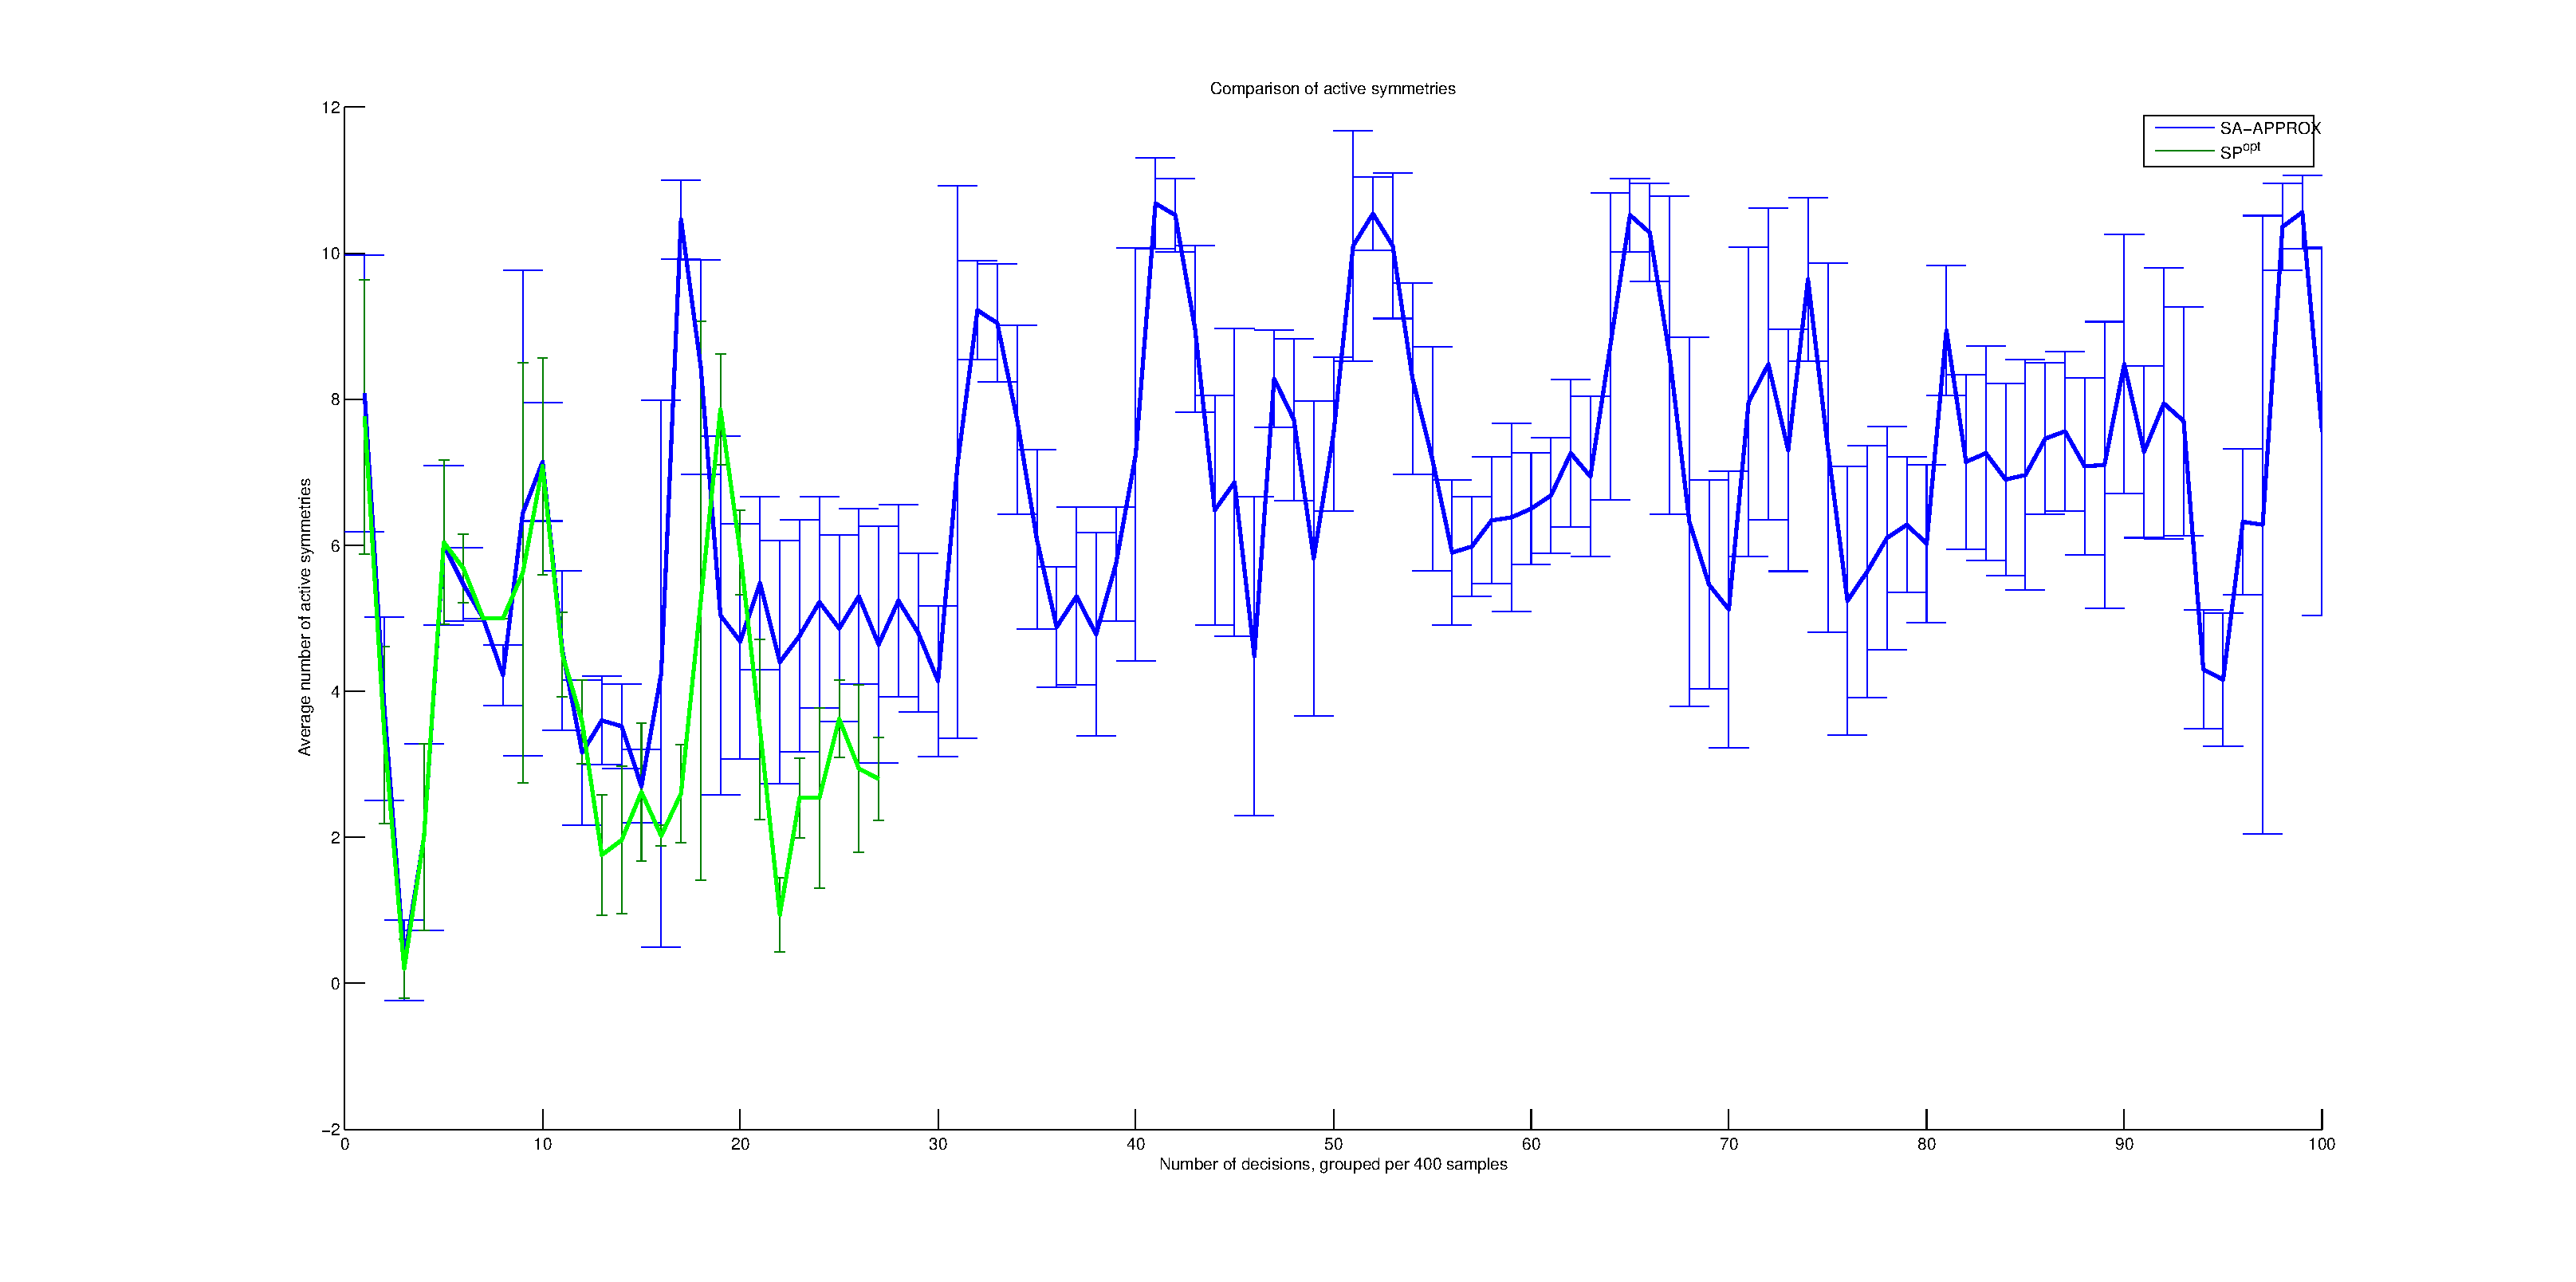
\includegraphics[width=1.2\textwidth]{results/battleship-12-23-approx-vs-reg.eps}}
		\caption{
			Number of active symmetries during search for one of the cases where SA-APPROX got
			outperformed by $SP^{OPT}$.
			We averaged over sample points; the error bars show the standard error on these
			averages.
			The specific case under test is battleship-12-23
		}
		\label{fig:active_symmetries_during_search}
	\end{figure*}

	Secondly, we have to consider that the implemented heuristics might collide with the built-in
	VSIDS heuristic, which is an important heuristic that dramatically increases search efficiency.
	SA and SA-APPROX however, only consider the top 5 variables on the variable heap, whereas VSIDS
	takes the first.
	This is a relatively small number considering the amount of variables in the instances,
	which means that variables rated high by VSIDS, are rated high by SA and SA-APPROX.

	Lastly, the result obtained by \cite{devriendt2012symmetry} should be considered.
	They implemented a heuristic based on the same hypothesis and obtained promising results.
	We note however, that only very datapoints verify that their heuristic on inverting symmetries
	yields better results (only the xorchain and urquhart sets contain inverting symmetries), and
	both SA and SA-APPROX showed increased performance (decision-wise) on Urquhart.
	These datapoints are not enough to support the hypothesis that higher symmetry activity, yields
	better performance.
